%% NSF XPS Proposal 2013

\documentclass{acm_proc_article-sp}

\usepackage{color}
\usepackage{graphicx}
\newcommand{\TODO}[1]{\textcolor{red}{{\bf TODO:} #1}}
\newcommand{\checkme}[1]{\textcolor{red}{\textbf{#1}}}




\begin{center}
  \textbf{\Large XPS-CLCCA: Scalable Parallelism for Irregular and Graph Applications}\\ \vspace{5mm}
  \textbf{Luis Ceze ~~~~~ Simon Kahan ~~~~~ Mark Oskin (PI)}\\
  \textbf{University of Washington}
\end{center}

\section{Introduction}

Irregular applications generate tasks with work, dependences, and memory
accesses that are highly sensitive to input. Classic examples of irregular
applications include branch and bound optimization, SPICE circuit simulation,
contact algorithms in car crash analysis, and network flow. Important
contemporary examples include processing large graphs in the business,
national security, machine learning, data-driven science, and social network
computing domains. For these emerging applications, fast response -- given the
sheer amount of data -- requires multinode systems. The most broadly available
multinode systems are those built from x86 commodity computing nodes
interconnected via ethernet or infiniband. Our focus is to enable scalable
performance of irregular applications on these mass market systems,
addressing two key challenges:

\paragraph{Irregular applications exhibit little spatial locality.} It is not atypical for any given task's data references to be spread randomly across the entire memory of the system. This makes current memory hierarchy features ineffective. Caches are of little assistance with such low data re-use and spatial locality. Commodity prefetching hardware is effective only when addresses are known many cycles before the data is consumed or the accesses follow a predictable pattern, neither of which occurs in irregular applications. As a consequence, commodity microprocessors stall often when executing irregular applications.

\paragraph{Irregular applications frequently request small amounts of off-node data.} On multinode systems, the challenges presented by low locality are analogous, and exacerbated by the increased latency of going off-node. Irregular applications also present a challenge to mass market network technology, which is designed to transfer large blocks of data, not the word-sized references emitted by irregular application tasks. Injection rate into the network is insufficient to utilize wire bandwidth when blocks are below about two-kilobytes, so any straightforward communication strategy severely under-utilizes the network.

%% I don't think we need the parahraph below. 
% While some irregular applications can be restructured to better exploit
% locality, aggregating requests to increase message size, and manage the
% additional challenges of load balance and synchronization across multinode
% systems, the work to do so is formidable and requires knowledge and skills
% pertaining to distributed systems far beyond those of most application
% programmers.

Luckily, many of the important irregular applications naturally offer large
amounts of concurrency. This immediately suggests taking advantage of
concurrency to tolerate the latency of data movement. The fully custom Tera
MTA-2~\cite{tera:mta1} system is a classic example of supporting irregular
applications by using concurrency to hide latencies. It had a large
distributed shared memory with no caches. On every clock cycle, each processor
would execute a ready instruction chosen from one of its 128 hardware thread
contexts, a sufficient number to fully hide memory access latency. The network
was designed with a single word injection rate that matched the processor
clock frequency and sufficient bandwidth to sustain a reference from every
processor on every clock cycle. Unfortunately, while an excellent match to
extremely irregular applications, the MTA was not cost-effective on
applications that could exploit locality and had very poor single-thread
performance, making it a commercial failure. The Cray XMT approximates the
Tera MTA-2, substantially reducing its cost but not overcoming its narrow
range of applicability.

In this proposal we first describe our early
Grappa prototype, a runtime system for irregular
applications. It provides several facilities: a global shared memory
abstraction, user-level threading support, and communication and
synchronization primitives. Applications targeted for Grappa are not expected
to have \emph{any} locality (although what locality that exists is favorably
exploited), but are expected to provide many thousands of concurrent threads.

Next, we present some preliminary results. Even as an early prototype, Grappa
runs several graph-crunching applications (classic examples of irregular
behavior) efficiently on a commodity cluster. For unbalanced tree search,
Grappa is over 3X faster and shows greatly improved scalability compared to
the Cray XMT; conversely, for breadth first search Grappa is 2.5X slower --
fast compared to implementations without Grappa, but obviously there is room
for improvement. Most importantly, however, for significantly less real world
cost, users can \emph{add} significantly more processors to a commodity
cluster than an XMT machine and use Grappa to achieve scalable performance.

Given these very positive early results,
we next propose to extend Grappa in the following directions:

\begin{itemize}

\item \textbf{Reinvent network communication:} Our preliminary work has
revealed limitations of the current Grappa runtime system with regards to
network scaling. This proposal plans to enhance the network layer with new
forms of communication scheduling and aggregation, and explore new forms of
hardware/software interactions of remote direct memory access (RDMA).

\item \textbf{Language and compiler support:} Presently, Grappa is implemented
strictly as a library.  A significant research thrust of the proposed work is to use
language and compilation support to provide a cleaner programming model and use
statically-available knowledge to lessen the runtime overhead automatically.

\item \textbf{Comprehensive benchmark suite:} Presently there does not exist a
comprehensive benchmark suite of irregular and graph applications. We
are also seeking funding through this proposal to put together just
such a benchmark suite. This suite will include benchmarks, reference
implementations, and input data-sets. In addition a website will be
created to distribute freely the benchmark suite and publish results.

\item \textbf{Support for \ssd\ only memory systems:} The size of data being
processed by large systems today (hundreds of terabytes) dwarfs what can fit
into a single system. Multiple system nodes are required to maintain and
access all of this data efficiently. However, even with hundreds of channels
to persistent storage, loading this data into DRAM can prove a bottleneck. The
Grappa runtime is designed to make applications tolerate extremely high memory
latency, thus we will explore using solid state disks as main memory, 
further taking advantage of Grappa's latency tolerance properties.


\end{itemize}

Finally, we propose to explore how the lessons learned performing this research -- specifically knowledge of what ultimately limits Grappa's performance for irregular applications using x86 processors and commodity networks with modified communication protocols -- can be applied to the design of future architectures.  Doing so will include studying the following research questions:

\begin{itemize}
\item \textbf{What is the right system architecture support for irregular applications, including architecture, communication and storage?}
\item \textbf{What are the necessary language and compiler support for large-scale, data-intensive irregular applications?}
\item \textbf{How do we comprehensively evaluate performance of graph analytics systems?}
\end{itemize}

\paragraph{Intellectual Merit:}

Efficiently executing irregular computations on commodity hardware is \emph{hard}.  Much about commodity hardware is seemingly designed for the opposite application characteristics: caches assume applications have locality; networks are built with low injection rates but high bandwidth, assuming large packet sizes; even runtimes and operating systems are built assuming relatively infrequent communication and synchronization compared to computation.  This proposal rests on the seemingly outlandish claim that this commodity hardware / software stack can be coerced, through another layer of software, into efficiently executing irregular applications that both lack locality and communicate frequently with small amounts of data.  A folksy way of saying it is we think we can jam a square peg through a round hole.  Fortunately we have some preliminary evidence we won't get wedged along the way.  This is an intellectually challenging endeavor, landing squarely in the middle of the NSF XPS program: using and exploiting parallelism from irregular computations to efficiently execute them at scale.

\paragraph{Broader Impact:}

Irregular computations are of increasing economic importance.  Moreover, they are key to several national security applications.  If commodity hardware can be cajoled into executing such applications efficiently it will open the door for new and rich applications.  Graph queries, machine-learning and data-driven science will be enabled by the technology we aim to create from the ideas in this grant proposal.  In addition our work will include the construction of a comprehensive irregular benchmark suite, something to help guide our own and the field's research.

%% Roadmap

\section{Description of the Current Grappa System}

In the twenty years that have elapsed since the Tera MTA, commodity microprocessors have become much faster and multicore has driven down the absolute price of computation; commodity network price-performance has improved as well. This shift has afforded us the opportunity to attack the challenges posed by irregular applications by emulating in software and inexpensive mass market hardware, the approach taken by Tera. We exploit the increased aggregate instruction rate per socket relative to chip bandwidth, using what would otherwise be wasted instructions to manage the multiplexing of as many as several thousand tasks per core, thus tolerating memory latency, reducing stalls, and making better use of available bandwidth. Ultimately, the opportunity is to cover the spectrum of irregular to regular computation: where tasks exhibit locality, multiplex fewer tasks and expend fewer instructions on context switching; where locality is lacking, multiplex more tasks at a higher rate to tolerate latency. Thus we make the best use of task parallelism -- either to scale to more cores or to tolerate latency -- and of caches -- either to exploit application locality or to house more task contexts.

Grappa is a software runtime system that allows a commodity x86 distributed-memory HPC cluster to be programmed as if it were a single large shared-memory machine and provides scalable performance for irregular applications. Grappa is designed to smooth over some of the performance discontinuities in commodity hardware, giving good performance when there is little locality to be exploited while allowing the programmer to exploit it when it is available.

Grappa leverages as much freely available and commodity infrastructure as possible. We use unmodified Linux for the operating system and an off-the-shelf user-mode infiniband device driver stack~\cite{OFED}. MPI is used for process setup and tear down. GASnet~\cite{gasnet} is used as the underlying mechanism for remote memory reads and writes using active message invocations. To this commodity hardware and software mix Grappa adds three main software components: (1) a \emph{lightweight tasking\/} layer that supports a context switch in as few as 38ns and distributed global load balancing; (2) a \emph{distributed shared memory\/} layer that supports normal access operations such as \emph{read\/} and \emph{write\/} as well as synchronizing operations such as \emph{fetch-and-add\/}~\cite{fetchandadd}; and (3) a \emph{message aggregation\/} layer that combines short messages to mitigate the aforementioned problem that commodity networks are designed to achieve peak bandwidth only on large packet sizes, yet irregular applications tend to fetch only a handful of bytes at a time. As we will show later, Grappa can tolerate latencies way beyond that of the network. Therefore, Grappa can afford to \emph{trade latency for throughput\/}: by {\em increasing\/} latency in key components of the system we are able to increase our effective random access memory bandwidth (by delaying and aggregating messages), our synchronization bandwidth (by delegating operations to remote nodes), and our ability to improve load imbalance (work stealing increases latency).

\begin{figure}[t]
\begin{center}     
  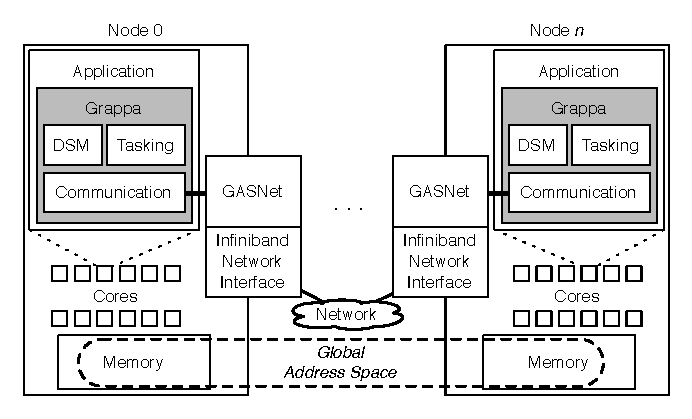
\includegraphics[width=0.95\columnwidth]{figs/system-overview}
\begin{minipage}{0.95\columnwidth} 
  \caption{\label{fig:grappa} Grappa system overview}
\end{minipage}
\vspace{-3ex}
\end{center}
\end{figure}

The current Grappa prototype (Figure~\ref{fig:grappa}) has three main software components: \begin{description}

\item [Tasking system.] Our tasking system supports lightweight multithreading to tolerate communication latency and global distributed workstealing (i.e., tasks can be stolen from any node in the system), which provides automated load balancing.

\item[Distributed shared memory.] Our DSM system provides support for fine-grain access to data anywhere in the system. It supports synchronization operations on global data, explicit local caching of any memory in the system, and support for operation on remote data (delegating operations to home node). By tight integration with the tasking system and the communication layer, our DSM system offers high aggregate random access bandwidth for accessing remote data.

\item[Communication layer.] As discussed earlier, modern commodity networks support high bandwidth only for large messages. Since irregular applications tend to need frequent communication of small requests, the main goal of our communication layer is to aggregate small messages into large ones to better exploit what the network can offer. It is largely invisible to the application programmer.

\end{description}

\subsection{Tasks}

The basic unit of execution in Grappa is a {\em task}. Each task is represented by a function pointer and its arguments. A new task is enqueued at spawn time; when resources are free, it is allocated a stack, bound to a core, and executed.

During execution, a task yields control of its core whenever it performs a long-latency operation, allowing the processor to remain busy while waiting for the operation to complete.  In addition,  a programmer can direct scheduling explicitly via the Grappa API calls. To minimize yield overhead, the Grappa scheduler operates entirely in user-space and does little more than store register state of one task and load that of another. Context switch times are as low as 38ns even when switching amongst thousands of tasks.

\subsection{Expressing parallelism}

Grappa programmers focus on expressing as much parallelism as possible without concern for where it will execute. Grappa then chooses where and when to exploit this parallelism, scheduling as much work as is necessary on each core to keep it busy in the presence of system latencies and task dependences.

Grappa provides two methods for expressing parallelism. First, when the programmer identifies work that can be done in parallel, the work may be wrapped up in a function and queued with its arguments for later execution using a \texttt{spawn}. A programmer can further specify using \texttt{spawn\_on} to spawn a task on a specific core in the system or at the home core of a particular memory location. Second, the programmer can invoke a parallel for loop, provided that the trip count is known at loop entry. The programmer specifies a function pointer along with start and end indices and an optional threshold to control parallel overhead. Grappa does {\em recursive decomposition} of iterations, similar to Cilk's cilk\_for construct~\cite {cilkforimplementation} and TBB's {\tt parallel\_for}~\cite{intel_tbb}.  It generates a logarithmically-deep tree of tasks, stopping to execute the loop body when the number of iterations is below a specified threshold.

\subsection{Memory}

Applications written for Grappa utilize two forms of memory: local and global.  Local memory is local to a single core in the system.  Accesses occur through conventional pointers.  The compiler emits an access and the memory is manipulated directly.  Applications use local accesses for a number of things in Grappa: the stack associated with a task, accesses to localized global memory in caches (see below), and accesses to debugging infrastructure that is local to each system node.  Local pointers cannot access memory on other cores, and are valid only on their home core.

Large data that is expected to be shared and accessed with low locality is stored in Grappa's global memory. All global data must be accessed through calls into Grappa's API. %, shown in Figure~\ref{fig:accessing-memory}.

\paragraph{Global memory addressing} Grappa provides two methods for storing data in the global memory. The first is a distributed heap striped across all the machines in the system in a block cyclic fashion. The \texttt{global\_malloc} and \texttt{global\_free} calls are used to allocate and deallocate memory in the global heap.  Addresses to memory in the global heap use \textbf{linear addresses}.  Choosing the block size involves trading off sequential bandwidth against aggregate random access bandwidth. Smaller block sizes help spread data across all the memory controllers in the cluster, but larger block sizes allow the locality-optimized memory controllers to provide increased sequential bandwidth. The block size, which is configurable, is typically set to 64 bytes, or the size of a single hardware cache line, in order to exploit spatial locality when available. The heap metadata is stored on a single node. Currently all heap operations serialize through this node; while this has been sufficient for our benchmarks, in the future Grappa will provide parallel performance through combining~\cite{MAMA,flatcombining}.

Grappa also allows any local data on a core's stacks or heap to be exported to the global address space to be made accessible to other cores across the system. Addresses to global memory allocated in this way use \textbf{2D global addresses}.  This uses a traditional PGAS addressing model, where each address is a tuple of a rank in the job (or global process ID) and an address in that process. The lower 48 bits of the address hold a virtual address in the process. The top bit is set to indicates that the reference is a 2D address (as opposed to linear address). This leaves 15 bits for network endpoint ID, which limits our scalability to $2^{15}$ endpoints. Any node-local data can be made accessible by other nodes in the system by wrapping the address and node ID into a 2D global address. This address can then be accessed with a delegate and can also be cached by other nodes. At the destination the address is converted into a canonical x86 address by replacing the upper bits with the sign-extended upper bit of the virtual address. 2D addresses may refer to memory allocated from a single processes' heap or from a task's stack.

\paragraph{Global memory access} There are two general approaches Grappa applications use to {\emph access} global memory. When the programmer expects a computation on shared data to have spatial locality to exploit, {\em cache} operations may be used. When there is no locality to exploit, {\em delegate} operations are used.

\textbf{Explicit caching.} Grappa provides an API to fetch a global pointer of any length and return a local pointer to a cached copy of the global memory.  Grappa cache operations have the usual read-only and read-write variants, along with a write-only variant used to initialize data structures. Languages for distributed shared memory systems have done optimizations to achieve a similar goal. For example, the UPC compiler coalesces struct and array accesses into remote get/put \cite{Chen:2005}, and Fortran D compiler's message vectorization hoists small messages out of a loop \cite{FortranD:1992}. Caching in Grappa additionally provides a mechanism for exploiting temporal locality by operating on the data locally.

Under the hood, Grappa performs the mechanics of gathering chunks of data from multiple system nodes and presenting a conventional appearing linear block of memory as a local pointer into a cache. The strategy employed is to issue all the constituent requests of a cache access request  (as Active Messages) and then yield until all responses have occurred.  Currently, Grappa caches are \emph{not} coherent, requiring the programmer to maintain consistent access to data.  Future work will develop a software directory based coherence scheme to simplify consistent access to global data.

\textbf{Delegate operations.} When the access pattern has low-locality, it is more efficient to modify the data on its home core rather than bringing a copy to the requesting core and returning it after modification. Delegate operations provide this capability. Applications can dispatch computation to be performed on individual machine-word sized chunks of global memory to the memory system itself (e.g., \emph{fetch-and-add}).  Delegate operations, proposed in \cite{Nelson:hotpar11} and \cite{delegated:oopsla11}, are also the primary synchronization method in Grappa.

Delegate operations are always executed at the home core of their address, and while arbitrary memory operations can be delegated, we restrict the use of delegate operations in three ways to make them more useful for synchronization. First, we limit each task to one outstanding delegate operation to avoid the possibility of reordering in the network. Second, we limit delegate operations to operate on objects in the 2D address space or objects that fit in a single block of the linear address space, so they can be satisfied with a single network request. Finally, no context switches are allowed while the data is being modified. Given these restrictions, we can ensure that delegate operations for the same address from multiple requesters are always serialized through a single core in the system, providing atomic semantics without using atomic operations. 

\subsection{Communication}
\label{sec:communication}

In order to mitigate the low message injection rate limits of commodity networks, Grappa's communication stack has two layers: one for user-level messages and one for network-level messages.

At the upper layer, Grappa implements asynchronous active messages \cite{vonEicken92}. Each message consists of a function pointer, an optional argument payload, and an optional data payload. When a task sends a message, the message is copied to a send queue associated with the message's destination and the task continues execution.

Grappa's lower networking layer aggregates the upper layer's messages to improve performance. Commodity networks including infiniband achieve their peak bisection bandwidth \emph{only} when the packet sizes are relatively large---on the order of multiple kilobytes. The reason for this discrepancy is the combination of overheads associated with handling each packet (in terms of bytes that form the actual packet, processing time at the card and processing on the CPU within the driver stack). Our measurements confirm manufacturers published data~\cite{infinibandbandwidth}, that with this packet size the bisection bandwidth is only a small fraction, less than 3\% of the peak bisection bandwidth.

In our experiments the vast majority of requests were smaller than 44 bytes, far too small to make efficient use of the network. To make the best use of the network, we must convert our small messages into large ones. When a task sends a message, it is not immediately sent, but rather placed in a queue specific to the destination.

There are three situations in which a queue of aggregated messages is sent. First, each queue has a message size threshold of 4096 bytes, chosen to give reasonable network performance. If the size in bytes of a queue is above the threshold, the contents of the queue are sent immediately. Second, each queue has a wait time threshold ($\approx${1ms}). If the oldest message in a queue has been waiting longer than this threshold, the contents of the queue are sent immediately, even if the queue size is lower than the message size threshold.  Third, queues may be explicitly flushed in situations where the programmer wants to minimize the latency of a message at the cost of bandwidth utilization.

The network layer is serviced by polling. Periodically when a context switch occurs, the Grappa scheduler switches to the network polling thread. This thread has three responsibilities. First, it polls the lower-level network layer to ensure it makes progress. Second, it deaggregates received messages and executes active message handlers. Third, it checks to see if any aggregation queues have messages that have been waiting longer than the threshold; if so, it sends them.

Underneath the aggregation layer, Grappa uses the \gasnet~communication library~\cite{gasnet} to actually move data. All interprocess communication, whether on or off a cluster node, is handled by the \gasnet~library. \gasnet~is able to take advantage of many communication mechanisms, including ethernet and infiniband between nodes, as well as shared memory within a node.

Some networks provide access to a remote machine's memory directly. This would seem to be a good fit for a programming model focused on global shared memory, but in fact we do not use it. In our experiments, we found that RDMA operations are subject to the same message rate limitations as all other messages on these cards, and thus using raw RDMA operations for our small messages would make inefficient use of bandwidth. Instead, we implement remote memory operations with active messages. A byproduct of this design decision is that Grappa is not limited to RDMA-capable networks.

\subsection{Performance}

To evaluate Grappa's performance with respect to the XMT, we ran each of our three benchmarks on up to 16 nodes of each machine. Grappa used 6 cores per node, with the best parameters chosen for each point. In some cases, the XMT could not run the benchmark with 2 nodes, so the point is omitted.

\begin{figure}
\begin{center}

\hspace{-1in}\begin{minipage}{0.3\textwidth}
\begin{center}
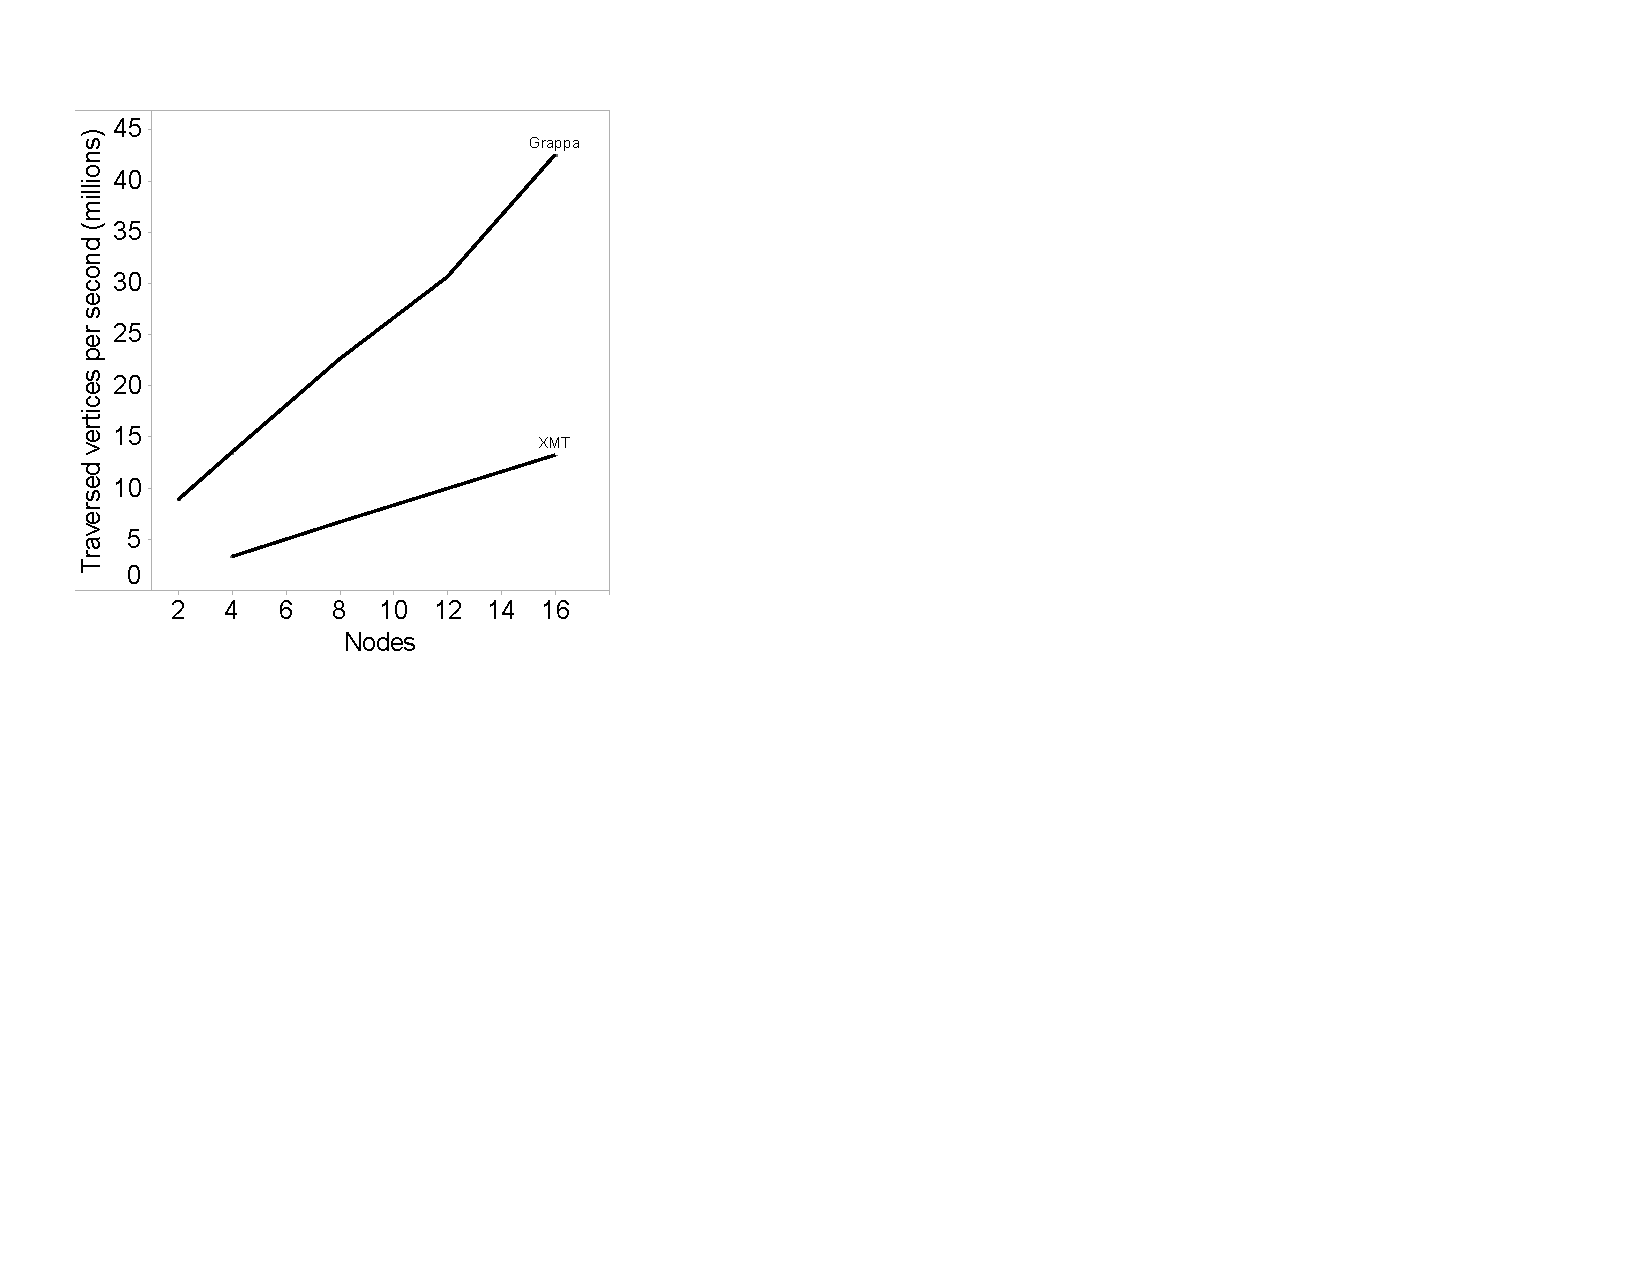
\includegraphics[width=3in]{figs/uts_performance.pdf}
\caption{\label{fig:uts_compare} Performance of in-memory unbalanced tree search.}
\end{center}
\end{minipage}
\hspace{1.25in}\
\begin{minipage}{0.3\textwidth}
\begin{center}
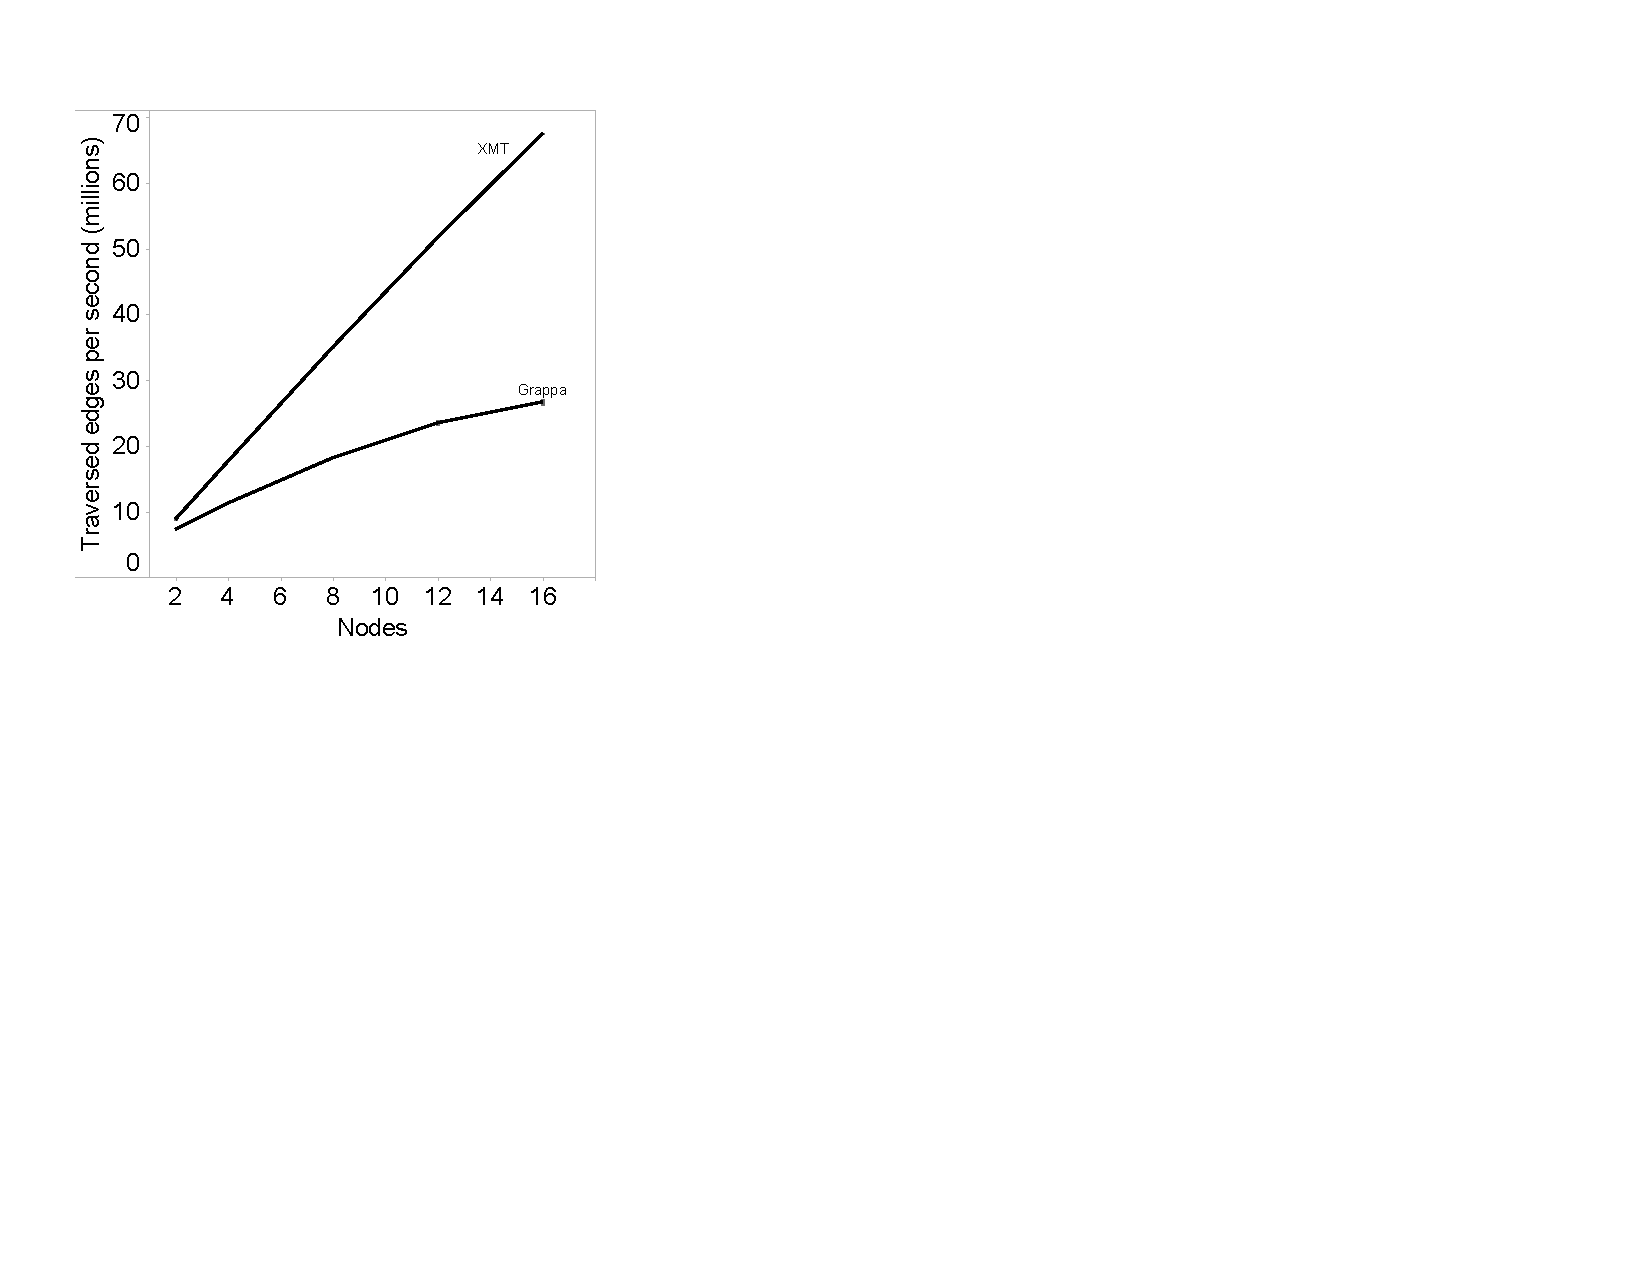
\includegraphics[width=3in]{figs/bfs_performance}
\caption{\label{fig:bfs-performance} Performance of breadth-first searcch.}
\end{center}
\end{minipage}

\end{center}
\end{figure}

\paragraph{Unbalanced tree search} We ran UTS-mem with a geometric 100M-vertex tree (T1L). Figure~\ref{fig:uts_compare} shows the performance in terms of number of vertices visited per second versus number of compute nodes. Grappa is 3.2 times faster than the XMT at 16 nodes.  As we will show later, the performance advantage Grappa has over XMT increases as more nodes are added.  The main reason Grappa performs better is the software-based delegate synchronization obviates the need for the retry-based synchronization that XMT uses.


\paragraph{BFS} We ran BFS on a synthetic Kronecker graph with $2^{25}$ vertices and $2^{29}$ edges (25 GB of data). Figure~\ref{fig:bfs-performance} shows our performance in terms of graph edges traversed per second. The XMT is 2.5 times faster than Grappa at 16 nodes.  Performance does scale at a constant rate for Grappa, suggesting that adding more nodes will increase performance.


\section{Related work}

Our efforts are built on many existing ideas in programming languages, systems and architecture. In this section we discuss related frameworks and key enabling technologies that Grappa builds upon.

\paragraph{Comparable frameworks} Distributed graph processing frameworks like Pregel~\cite{pregel:2010} and Distributed GraphLab~\cite{distgraphlab:vldb12} share similar goals as Grappa. Pregel adopts a bulk-synchronous parallel (BSP) execution model, which makes it inefficient on workloads that could prioritize vertices. GraphLab, on the other hand, schedules vertex computations individually, allowing prioritization, which gives faster convergence in a variety of iterative algorithms.  GraphLab, however, imposes a rigid computation model where programmers must express computation as transformations on a vertex and its edge list only, with information only from adjacent vertexes. Pregel is only slightly less restrictive, as the input data can be any vertex in the graph.  Grappa also supports dynamic parallelism with asynchronous execution, but parallelism is expressed as tasks or loop iterations, which is a far more general programming model for irregular computation tasks.

\paragraph{Global memory} Grappa includes a custom implementation of a software distributed shared memory (DSM) system. Many traditional software DSM systems are page based~\cite{Treadmarks,munin} and aim to hide the fact that they are built in software from applications by exploiting the processor's paging mechanisms, therefore relying heavily on locality. Instead, Grappa, like other partitioned global address space (PGAS) models, implements its DSM at the language, rather than system level. Languages such as Chapel~\cite{Chamberlain:2007}, X10~\cite{X10:2005}, and UPC~\cite{upc:2005} make accesses to shared structures look like normal memory references. As we describe later, Grappa chooses a middle ground, where global addresses are explicit in the API and local accesses are emitted conventionally by the compiler.  While Grappa's DSM system is conceptually similar to prior work, its implementation is tuned for irregular computations.  Past DSM work, being page-based, could exploit the RDMA capabilities of network hardware to move large page-sized blocks of data from node to node. In our experience, when these networks move small blocks of data (a few bytes), only a fraction of the available bandwidth is achieved. In addition, the DSM system in Grappa ends up being tightly coupled to the task scheduler in order to overlap long latency memory operations with useful computation.  For these two reasons it became necessary to build a new DSM system specifically for Grappa.

\paragraph{Multithreading} Grappa uses multithreading to tolerate memory latency. This is a well known technique. Hardware implementations include the Tera MTA~\cite{tera:mta1}, Cray XMT~\cite{feo:xmt}, Simultaneous multithreading~\cite{tullsen:smt}, MIT Alewife~\cite{agarwal:alewife}, Cyclops~\cite{almasi:cyclops}, and even GPUs~\cite{gpus}. As we describe in this paper, Grappa use a lightweight user-mode task scheduler to multiplex \emph{thousands\/} of tasks on a single processing core. The large number of tasks is required because of the extremely high internode latency Grappa is mitigating.  Grappa's task library employs several optimizations: an extremely fast task switch, a small task size, and judicious use of hardware prefetching to bring task state into the cache long before that task is actually scheduled.

\section{Proposed Research}

As described earlier, our work on Grappa so far has focused on building an initial prototype so we have a baseline system to build upon. This early prototype has lead us to think of many research opportunities, from new ways to improve network communication scheduling, to new data storage management ideas to compiler and language support. Below we detail our research plans in each of these thrusts. 

\subsection{Networking}

Since Grappa is designed for applications that have no or low locality, nearly \emph{every} memory reference is to a remote system node.  This makes the networking layer key to overall system performance.  In this section we outline the key directions we wish to take in enhancing the networking layer of the Grappa runtime system.

\paragraph{Virtual topology:} Currently Grappa uses a flat network topology where each processing core in the system is individually addressed. As more nodes are added to the system, a quadratic increase in the number of threads (in aggregate across all nodes) is required in order to compensate for the \emph{same} network delay.  This is because the current aggregator treats each of these end-points individually, i.e., it only aggregates messages that go to the same exact end-points. This does not scale as the number of nodes increases because the probability of messages going to the same destination goes down (assuming a somewhat uniform communication distribution). In summary, this past design choice is simple but does not scale.

We need to rewrite the aggregator to build in a hierarchical virtual network layer.  The first layer of this hierarchy is to treat all processors at a given system node as a single destination. We intend to continue to use the lock-free single-threaded \gasnet~communication layer that we have been using, as we have found the lock-based one to incur too high of an overhead for our purposes.  Thus the aggregator will need to very carefully utilize lock-free data-structures and interact with \gasnet~carefully.

The second, and upper layers of the virtual topology are built from clustering system nodes into groups.  Instead of aggregating for all end-points, aggregation will occur for system nodes within a group.  A designated (and dedicated) node will act as a router, processing incoming and outgoing traffic to system nodes within the group and other groups.

We expect this hierarchical organization will reduce scaling requirements from
\BigO{n^2} threads to \BigO{n \times log(n)}. Of course, it takes what used to
be a single network hop for communication and turns it into \BigO{log(n)}
hops. More threads will be required to overcome this increased latency, but we
hypothesize only \BigO{log(n)} more, hence a real \BigO{n / log(n)^2} scaling
benefit is achievable with a virtual hierarchical network topology. 

\paragraph{Hardware support for aggregation:} If the increased latency caused
by extra hops in hierarchical aggregation turns out to be detrimental, we
will explore mitigation by moving some of the aggregation logic to the network
card, either by exploiting off-the-shelf programmable network cards or
experimental systems such ask NetFPGA~\cite{netfpga} (while we are planning to
focus on Infiniband-based networking, if we explore the NetFPGA route we will
be using Ethernet).

\paragraph{User-level RDMA:} Certain commodity networking hardware today
supports remote direct memory access (RDMA). Unfortunately, \emph{how} it is
implemented is so primitive and low-level that it is difficult or impossible
to efficiently use in practice. We start with a short description of the
current semantics of RDMA implementations. Next we describe the research we
wish to undertake to make RDMA more useful.

Networking infrastructure supports remote read and write operations.  Read operations take a source address and key (on a remote node), a destination address and key (on the local node), and a length.  Cards support address translation for regions of memory that are registered with them.  These translations, indexed by the supplied key, are used to perform virtual to physical address translation.  The physical address of the destination address is similarly translated using the translation table at the local node.  Cards also support remote write operations with a similar set of semantics, where addresses are translated on a card using the card's local translation table.  Both read and write operations are asynchronous.  The requesting processor initiates the operation and then can check for completion by querying a completion queue at the local card.  \emph{Notably}, the processor(s) on the remote node are provided a polling interface whereby they can learn if a remote write operation occurred.  No such interface exists to learn about remote read or atomic operations.

This interface suffers from multiple shortcomings.  The biggest of which is that ultimately, moving data to and from a remote node constructively requires higher level semantic operations than simple reads and writes.  These higher level semantics can, of course, be synthesized from the underlying read and write primitives, but it wastes round trips and synchronization time.  One possible alternative solution is to enable remote nodes to dispatch high-level data-structure manipulation requests (e.g. insert this item into a queue, remove an item from a set).  The challenge here is to make those calls programmable and interoperate securely with a modern operating system, and a user-level runtime system.  Additionally there are questions about \emph{who} should carry out the computation.  Classic RDMA does not interrupt the host processor, but these richer programmable semantics will require either a processor in the network interface (necessitating issues such as coherence be managed) or complex RDMA tasks need a mechanism to interrupt the host processor \emph{without leaving user space}. 


%% The second half of this paragraph is really confusing, I have just a minimal clue of what it is talking about. And the little I understand sounds a bit vague and not directly related to grappa.
The second challenge is that the virtual to physical address translation on the cards requires the operating system to pin translations.  This removes paging flexibility from the operating system, because runtime systems are (rationally) built to expect data structures to be in memory capable of RDMA or not.  Those in RDMA memory must be pinned.  In the long run, the solution here likely lies at the intersection of what progress is occurring in processor support for virtual machines and virtual memory translation for I/O.  Our goal will be to study carefully the I/O virtualization proposals put forth by major processor manufactures and devise solutions that enable RDMA to capitalize on these developments.

\subsection{SSD-only data structures}

Grappa applications are likely to use large amounts of data, 100s of terabytes to petabytes. Keeping all these data in DRAM only is unlikely to be cost effective. We will explore mechanisms that use solid-state storage as primary memory, greatly expanding the directly addressible storage at low cost.

Grappa is very effective in hiding latencies of network communication.  If an access is to a chunk of the heap stored in a node's local memory, Grappa issues a prefetch for the address and context switches to other work while the prefetch is executing~\cite{Nelson:hotpar2011}. If the access is to memory stored on another node, Grappa issues a message to that node to request the data and context switches to other work until the reply arrives.  In fact, our measurements and estimates show that we might be able to tolerate even greater latency -- on the order of milliseconds per request.  This provides the tantalizing possibility that we will be able to keep data in \ssd\ drives only and service data access requests directly from them, without leaving copies in DRAM.  The natural point of integration for non-volatile memories in Grappa is to store the global distributed shared heap in non-volatile memory. All accesses to this shared heap are done through an \api, so this switch would be transparent to the programmer.

This is not straightforward, however, for three reasons: (1) \ssds\ assume spatial locality. In our benchmarks, we find the average request size to be less than 64 bytes. Today's \ssds\ are optimized for reads in the multi-kilobyte range. (2) \ssds\ have a low request rate. The fastest~\cite{fusionio} can perform on the order of 1 million random reads per second, and many are limited to less than 100K/s. Even the underlying flash chips are slow, on the order of 40K/s~\cite{micronFlash}. In contrast, our measurements suggest cores may be idle in Grappa if each node cannot perform 100 million random reads per second of the global heap. And (3) \ssds\ have high overhead. Mass market \ssds\ are usually treated as normal disks: accesses must occur through the kernel, incurring a high context-switch overhead. Grappa depends on user-mode access to the network layer to avoid this overhead; a similar approach has been applied to \ssds\ in recent research~\cite{caulfield:2012}, however.  We see several ways to address these challenges:

\paragraph{Scaling up the Flash array:} Existing Flash-based \ssds\ are designed for large block requests. An \ssd\ for Grappa could be designed to support high concurrency, small requests. Where a traditional \ssd\ might put multiple Flash chips on the same bus, or use Flash chips in parallel to build a wider, high-bandwidth bus, a Grappa \ssd\ would try to maximize message rate by putting each chip on its own bus. Serial Flash might be used to minimize pin count requirements, at the cost of some additional latency. This design could scale to our necessary request rates, but only at an enormously high chip count: to support 100 million reads per second, an array of 25$\mu$s flash would require 2500 chips.

\paragraph{Scaling down the processors:} Alternatively, rather than scaling up the flash array, processors could be scaled down to match the flash request rate. A low-power processor with few cores might generate only 1 million references per second. This could be satisfied with only $25\times 25\mu$s Flash chips. There are two problems with this design for our purposes, however. First, while each node requires fewer chips, the overall cluster performance goal, and thus chip count requirement, is the same. More system nodes are thus required to achieve the same level of performance.  Second, low single-threaded performance is detrimental to performance during periods of diminished application concurrency.

\paragraph{Buffering requests to increase locality:} Grappa trades latency for throughput by aggregating network communication. The same idea could be applied to increase locality and amortize the cost of Flash accesses. Requests to nearby flash locations would be bucketed by flash page address for a limited time. When a sufficient number of requests have arrived for a page or when the requests time out, a single page request would be issued to the Flash layer; its result would be used to satisfy the individual requests.  The challenge with this approach is as storage size grows, the effectiveness of aggregation correspondingly decreases.  On the other hand, aggregation occurs for all global memory requests generated by any node in the system, so as aggregate system performance increases, aggregation performance actually \emph{increases} (up to the point that the network is saturated).

%% Sorry Mark, while the item below is clearly rich and juicy, we can't leave it bhere because it is huuuuge, it does not match the scope of the grant, and we dont have the expertive --- e.g., are you sure nobody is working on it? 

%% I think this is the only idea that is going to work... maybe we should delete the above three and make this one good.  Seriously, the ideas up there are bunk.  -ark
% \paragraph{Rearchitecting flash:} Clearly the best solution here lays in re-architecting the flash chip itself.  We will explore new flash microarchitectures that optimize for message rate as well as bandwidth.  Such chips have value far beyond Grappa.  Research into persistent key/value stores, and really any persistent high-throughput data-structure will benefit from a redesigned flash chip that can sustain dramatically increased message rates.

\subsection{Compiler and language support}

Language and compiler support are instrumental in making Grappa usable to a wide audience of software developers. We envision language and compiler support can tackle a wide variety of challenges:

\paragraph{Relaxed consistency:} Presently Grappa uses a consistency model that is sequentially consistent for data-race free programs.  Underlying hooks are available to build even more relaxed consistency models, although we don't expect programmers themselves will want to use them.  A compiler, however, can see a performance boost by analyzing code and exploiting alias knowledge to program to this underlying Grappa \api, potentially gaining a performance boost by exposing more memory concurrency and hiding more latency.

\paragraph{Language support for synchronization operations: } At the moment, runtime library support is provided in Grappa for basic synchronization primitives (lock, barrier, etc).  Building synchronization directly into the language has the advantage that the compiler can understand and optimize it.  Several optimizations are possible in the Grappa framework, including exploiting the scheduler and work stealer to elide certain lock operations (scheduling is co-operative on a per-CPU basis), converting synchronization primitives into remote delegate operations, and exploiting the check-in / check-out nature of global memory in Grappa to coalesce multiple synchronization operations together.

\paragraph{Delayed writes: } At the moment when we we write applications for Grappa we use a technique that we call feed-forward delegates.  Essentially what this technique does is if a loop is reading and writing disjoint sets of data, it is possible and we have found efficient, to dispatch writes asynchronously and ensure those writes are completed only by the end of the loop.  This increases performance by further overlapping computation with memory access.  A compiler with alias analysis can do this transformation automatically for the programmer.

\paragraph{Automatic delegate synthesis: } Delegates are a technique in Grappa where one thread can request a small computation to be carried out on a remote node.  For instance, an increment on a memory location is dispatched to the system node that manages that memory operation and carried out there.  Currently the decision of what is a delegate is left to the programmer.  But this is an area rich for compiler optimization.  We will explore techniques to automatically synthesize delegates from code, potentially leading to more complex delegates and more efficient code.

\paragraph{Read and write combining: } As a special case of automatic delegate synthesis, when multiple remote memory operations are to be dispatched to the same node from the same thread, it may be more efficient to combine these together into a single request.  We will develop a compiler pass to combine operations when possible.

\paragraph{Compile for a continuation model: } Presently, whenever a task is active it is allocated a complete stack.  Since several thousand tasks are active per processor at any one time, these stacks occupy a large footprint in memory.  We wish to explore compiling tasks to a continuation model, whereby when a task dispatches a remote memory operation and is to be context-switched out, another task can utilize that stack.  Combined with the delegate synthesis ideas described above, we will also explore runtime and compiler support to convert remote memory operations into thread migrations; instead of moving the data to the system node that has the task, we will move the task to the data in cases where that would be more efficient.

\paragraph{Task-weaving: } Much of the time the same task code is executing for hundreds of thousands of tasks in the Grappa runtime system.  For example, each task may be processing a loop body for a parallel for loop.  However, tasks introduce overhead, so we already manually impose a cutoff on recursive decomposition of parallel loops.  This way, multiple loop bodies are collected into a single task and executed serially.  However, this limits the amount of parallelism available for latency tolerance. A mmore efficient technique is to allow the compiler to unroll and schedule all loop bodies simultaneously within the same task, including overlapping remote memory operations, thereby ``weaving'' these independent tasks together to overlap computation with communication with minimal task overhead.  Further, a set of ``woven tasks'' may be amenable to vector execution, allowing even more parallelism to be exploited.

\paragraph{Concurrency Control: } Having too few tasks multiplexed per core fails to tolerate fully the latency; having too many increases memory and cache footprints, resulting in excess cache misses or exhausting physical memory unnecessarily.  Currently, we choose a number at program instantiation:  experiments so far have shown evidence of a broad sweet-spot, though it is of course varies as a function of application behavior.  At compile-time, we could estimate the number of tasks required based on the density of remote operations and hard-coded measurements of system characteristics; at runtime we can adjust the number of tasks dynamically based on real-time measurement of processor counters.  Exploring these directions may lead to even more robust performance.

Presently we are starting work on this language and compiler support.  We are basing our effort on the LLVM~\cite{llvm} infrastructure.


\subsection{Graph benchmark suite}

In order to facilitate the development and evaluation of Grappa, we will develop a comprehensive benchmark suite for graph analytics applications. This will not only be useful for us, but the whole community at large, since there are few benchmarks in this application space.

This benchmark suite will consist of application kernels, reference implementations, data-sets, data-set generators, documentation, specifications for generating standardized performance results, and a hosting service (http://graphbench.org) to provide public access to the benchmark and datasets as well as aggregate and publish results by all users of the benchmark suite.

This benchmark suite will be a tremendous value to the research community. Not only will it enable researchers to evaluate ideas on graph processing system techniques, but it will also enable fair comparisons of ideas in a depth not currently available from other graph related benchmark suites~\cite{graph500}. The benchmark suite will be released in a completely open fashion, so anyone will be able to use it (and contribute to it).  All code will be distributed into the public domain (BSD style licensing) so companies can use it. The goal is to get something out relatively early in the hope of (i) getting others to cluster around this work rather than develop a plethora of overlapping alternatives, and (ii) help establish consistent metrics for performance results.

We will build a collection of key computational kernels from graph and irregular applications. The benchmark suite will consist of both documentation on the actual kernel (ideally a research paper or book reference sourced from the community), and a reference implementation. The benchmark suite will also include sample data collected from existing sources, and synthetic workload generators. The collected data provides a grounding for performance analysis on real-world problems. The workload generators provide cleaner, easier to reason about randomly generated data-sets at a programmable scale.

\section{Broader impacts}

\paragraph{Increasing involvement of underrepresented groups:} Computer science as a whole has a significant problem attracting women and minorities to the field.  Computer architecture has an even more extreme problem with diversity (in the PI's view).  This is a problem the PIs have taken quite seriously since entering the field, and we are quite proud of our PhD students, both female who have gone on to faculty positions in top academic institutions, and male who appreciate the gender and ethnic disparity and who work hard at their own institutions to correct it.  We continue to recruit a diverse graduate student mix and we continue to include undergraduate students in our research.  At the moment we are mentoring two women undergraduates involved in the Grappa project, and if this proposal is funded will apply for REU funds to continue their involvement.

\paragraph{Benchmark suite:} As previously described, we are seeking funding support to build and distribute a benchmark suite for irregular and graph applications.  This benchmark suite has the potential to have a broad impact on academia and industry.  We will distribute this benchmark through \texttt{graphbench.org} and will also collect and publish results from competing research groups.

\paragraph{Technology transfer:} Bill Dally during his 2010 Eckert-Mauchly award speech said (in effect), technology transfers happen when people transfer.  Having just come back from a three year stint founding a startup company (where we transferred the Deterministic Multiprocessing technology from UW), we've seen this first hand.  The students and faculty involved in the Grappa project plan to spin off a company with their work.  The exact time frame is not yet known, but everyone involved in the project is excited to see the technology underpin a startup company and make this technology available to the broader commercial world.

\paragraph{Curriculum development activities:} Concurrent with the execution of the research activities described in this grant we will seek to teach an advanced graduate class on advanced concurrency concepts.  We taught a similar class over six years ago and it is time to revive, update and teach it to the next generation of computer architecture graduate students.  \comment{Add more here.  This has no passion. -Mark}


\section{Results from Prior NSF Support}

\paragraph{Ceze:} Prof. Ceze's research is on computer architecture, programming languages and operating systems. His primary focus has been on improving programmability, reliability and energy efficiency of multiprocessor computer systems. His research is funded primarily by NSF, PNNL and industry. His CAREER award {\em Deterministic Shared Memory Multiprocessing: Vision, Architecture and Impact on Programmability} (CCF-0846004, 2008-13, \$559K) demonstrated that it is possible to provide deterministic execution of arbitrary multithreaded programs without sacrificing performance significantly. The results include innovation in architecture, compiler, and operating-systems. Two other NSF grants, {\em Code-Centric Approach to Specifying, Checking, and Discovering Shared-Memory Communication} (CCF-1064497, 2011-2014, \$901K) and {\em Precise Concurrency Exceptions: Architecture Support, Semantics and System Implications} (CCF-1016495, 2010-2013, \$500K), are leading to significant results in dealing with concurrency errors and concurrent programming language semantics. His work on large-scale graph processing is being funded by the Pacific Northwest Laboratory. His work on energy-aware programming models and approximate computing has been primarily funded by a seed NSF grant {\em Disciplined Approximate Programming for Energy-Efficient Computing} (CCF-1216611, 2012-2015, \$300K) and industry, including Microsoft, Google and Qualcomm.

\paragraph{Kahan:} Dr. Kahan's research has focused on irregular parallel computation.  Over the course of twelve years, he developed the Tera MTA's multithreaded runtime system and memory allocator still in use today in the Cray XMT, exploring applicability of the system to production codes and benchmarks in the engineering, science, and government domains.  His research has been driven by real-world application needs, resulting in new algorithms and systems to address concurrency bottlenecks.  He is presently an employee of the Pacific Northwest National Laboratory and an affiliate faculty member of the Computer Science and Engineering Department at the University of Washington.  He has no past or current NSF support.

\paragraph{Oskin:} Prof. Oskin's prior research has focused on architectures and systems for scalable computing.  With support from NSF he has carried out a variety of research activities, leading to over 50 scholarly publications, three PhD students graduated, four masters students graduated, and a company spin-off.  The past NSF-supported work (WaveScalar) heavily influences the ideas described here. In some sense, the work here is a culmination in thought processes about why WaveScalar did not achieve as much ILP as earlier limit studies in ILP suggested were possible.  NSF support for the PI's work, {\em ITR: WaveScalar, A New Approach to Scalable System Design} (CCF-0325635, 2003-07, \$1.3M), {\em CAREER: Soft-Instruction Set Computing} (CCF-0133188, 2002-05, \$443K), helped to develop WaveScalar.  He has also spent over a decade exploring architectural implications of quantum computing technologies, with support from NSF {\em NER: Computer Aided Design of Silicon-based Quantum Computers} (CCF-0210373, 2002-04, \$90K), {\em EMT: Microarchitectures for Quantum Computers} (CCF-0523359, 2006-10, \$275K), {\em EMT: Self-Correcting Fault-Tolerant Quantum Computers} (CCF-0523359, 2005-08, \$406K) DARPA {\em QuIST: Architectures and Applications for Scalable Quantum Information Systems}.  He is currently exploring runtime systems for irregular parallel applications, which is the subject of this proposal and is partially funded by the Department of Energy.

\section{Work Plan}
\label{sec:plan}

Our research plan can be divided horizontally into three core areas: programming languages/compilers; communication and storage; and benchmarking. Below we outline how we plan to advance these fronts over the next four years.

\vspace{2ex}


\noindent\textbf{Year 1:} The first year of this effort will focus on creating the benchmark suite and initial language and compiler support.  We aim to pull together 6-8 benchmarks, sample data sets, and scripts to measure performance results on the initial Grappa runtime, UPC~\cite{upc:2005} implementations, and serial reference code.  For the compiler we will have the front end done enabling easy addition of keywords to annotate data-types and structural elements (parallel for, etc).  The compiler will be generating in-efficient Grappa code by the end of the first year.

\vspace{1ex}
\noindent\textbf{Year 2:} The second year of effort will see the completion of the benchmark suite, a significant effort on compiler optimizations for Grappa, and the beginning of the networking layer research.  The benchmark suite will include 12-15 applications and/or kernels.  The website will be live and we will be conducting significant outreach efforts to drive adoption.  On the compiler front we will have implemented the key optimizations that provide the highest benefit for Grappa code.  In addition we will have a detailed understanding of what additional work remains to support other languages / language constructs.  In this year we will start work on rewriting the networking layer of the Grappa runtime, providing a virtual network topology.  We will also begin work on programmable RDMA by using FPGA-based networking gear.


\vspace{1ex}
\noindent\textbf{Year 3:} In the third and final year of this effort (supported by this grant), we will finish the networking layer rewrite.  We will also have constructed a test-bed system comprised of mainly SSD-based memory.  Grappa will be ported to this new style of memory, which we envision will largely be a tuning and not rewriting effort.  We will explore alternative SSD-memory designs largely through emulation.  Finally we will complete a detailed system evaluation using our benchmark suite.

\section{Summary}

Irregular applications are increasing in importance to the computing industry.  For a long time they have underpinned computations of interest to the national security arm of the federal government.  But now, they underpin such questions as ad placement in social networks, and analysis of complex data-sets in medicine and science.  The defining characteristic of these applications is poor locality and massive available parallelism.  Our effort is focused on making these applications perform well and scale on commodity hardware.  The ``secret sauce'' that makes this work is to essentially build a software XMT~\cite{feo:xmt}.  Instead of relying on locality (which doesn't exist for these applications) we rely on threading to tolerate memory latency.  Unlike the XMT, however, we must contend with commodity networking hardware, and here we again rely on threading to provide a sufficient number of requests that we can buffer them prior to dispatching on the physical wire.

Our past effort has shown a workable proof of concept of all this runtime smoke and mirrors: a commodity cluster can out do the XMT at its own game, by emulating its key features in software.  What is needed now is additional effort to improve the underlying performance of this runtime and make it usable to a broad base of developers.  We will be focusing our efforts in the next three years on the key performance component, the networking layer, and the key programmer efficiency linchpin, high level language support.  In addition we need a useful mechanism for handling data-sets in the petabyte range, and here we imagine building a cluster of machines that relies primarily on SSD's and not DRAM for data-set storage.

If successful, the Grappa runtime will have a transformative impact on the computing industry.  Irregular applications are hugely important, and if off the shelf hardware can be efficient with them a new class of questions can be asked of computing systems.  Additionally our benchmark suite development will further drive innovation among researchers in this space.


%%%%%%%%%%%%%%%%%%%%%%%%%%%%%%%%%%%%%%%%%%%%%%%%%%%%%%%%%%%%%%%%
%%%%%%%%%%%%%%%%%%%%%%%%%%%%%%%%%%%%%%%%%%%%%%%%%%%%%%%%%%%%%%%%
%%%%%
%%%%% Extra stuff: collaboration plan and data-management plan
%%%%%
%%%%%%%%%%%%%%%%%%%%%%%%%%%%%%%%%%%%%%%%%%%%%%%%%%%%%%%%%%%%%%%%
%%%%%%%%%%%%%%%%%%%%%%%%%%%%%%%%%%%%%%%%%%%%%%%%%%%%%%%%%%%%%%%%

\newpage

\section*{Data Management Plan}

The proposed research involves developing experimental systems and
assessing how well they work. The kinds of data we will produce
include: characterization data of program behavior; data on system
performance and reliability; data on how programmers use new language
constructs and tools. As is our practice, we will regularly submit
papers for publication detailing our findings and design of our
systems.

As we have already been doing with all our research, for every
published paper, we make all the raw data available online. This
allows other researchers to look at the data in different ways, and it
enables them to reproduce results. We also often publish
the experimental software developed, following the rules outlined by
the University intellectual property office --- which provides ample
rights for other researchers to build upon our experimental
systems. We do not anticipate using privileged or confidential
information. 

\newpage
\section*{Collaboration Plan}
%\setcounter{page}{1} 

Because the PIs already successfully collaborate and co-advise an
active cadre of spectacular students, the necessary tools and
coordination mechanisms are already in place for this project to
proceed successfully.  We first describe the PIs' complementary
backgrounds, then describe the current organization of our (amorphous)
research group, then describe the specific technology and facilities
that enable seamless coordination, and finally describe specific PI roles
for the research in this proposal.

\subsection*{Complementary PI Experience}

PI Oskin has traditionally participated in the computer-architecture research
community, co-PI Ceze, in addition to the architecture community also has a
presence in the systems and programming languages community, and co-PI Kahan
has participated mainly in the parallel and scientific computing community.
The move toward multicore architectures has re-invigorated collaboration
across these divides and recent joint work by Oskin, Ceze, and Kahan
embodies this important trend. There are currently five graduate students for
which last two of the PIs serve as advisors. In addition to the project
described in this proposal, they are working together on techniques for
detecting concurrency errors with machine learning and language
specifications, using disciplined approximations to save energy in computing,
and developing new operating-system abstractions for emerging non-volatile
memory devices. What has made these collaborations so fruitful in such a short
period of time is the PIs' complementary backgrounds. We now briefly describe
these backgrounds.

Oskin has... {\bf MARK PUT YOUR STUFF HERE.}

Ceze has been conducting research on architecture support, compiler
techniques, and programming models to improve the programmability of
multiprocessor systems for seven years and has co-authored over thirty
papers in these areas.  His research includes advances in
architecture~\cite{tlsooo, bulk, bulksc, swbulk, cyclops, dmp,
  delorean} and programming models~\cite{colorama, ipot, posh} to
simplify exploiting concurrency in multiprocessors. Some of his recent
results especially related to this proposal include a programming
model based on ordered transactions and data annotations~\cite{ipot};
improving reliability of multithreaded software with architecture
support for bug detection and avoidance~\cite{atomaid, aatoppicks,
  bugaboo, oshajava, cs-isca10, ce-isca10}; and deterministic
execution of multithreaded programs~\cite{dmp, dmptoppicks,
  asplos10coredet, dmpos}. PI Ceze recently co-organized an NSF-funded
workshop focused specifically on deterministic multiprocessing. The
workshop was very successful, bringing leaders in the multicore area
from industry and academia.

Kahan has been working in the area of parallel computing for irregular
applications for twenty years, largely in industry.  At Cray (previously Tera
Computer) he developed the runtime system~\cite{Alverson95schedulingon,Alverson97terahardware-software} and combining memory allocator~\cite{MAMA} still in production use on
Cray's XMT system in which over 50,000 threads execute concurrently sharing one
global address space.  He has co-authored patents and publications for both of these
systems as well as for a scalable connected components graph algorithm that bears
his name~\cite{Underwood07analyzingthe}.
Kahan originated and for three years has been co-PI for the Grappa project.

\subsection*{The SAMPA Research Group: Addressing the Concurrency
  Challenge Across the Execution Stack}

The PIs organize their joint research activity under the umbrella of
the ``SAMPA group'' (SAfe MultiProcessing Architectures).  Some brief
statistics help summarize the group's size, strength, and focus:
\begin{itemize}
\item There are roughly ten graduate students, most actively
  coadvised.
\item In the last four years, the group has produced twelve papers
  published in ASPLOS, ISCA, PLDI, OOPSLA, MICRO, and OSDI as well as three
  papers in the USENIX Workshop on Hot Topics in Parallelism.
\end{itemize}
The SAMPA group is an ideal size for collaboration across the system
execution stack from computer architecture up through software
engineering.  Compared to large collaborations with several faculty,
there are no graduate students (or faculty) who specialize entirely in
particular subtopics.  The students gain expertise across
computer-science disciplines and use appropriate ideas from hardware,
software, theory, etc. to solve research problems.  

\subsection*{Specific Technology and Facilities}

The research group that will perform the research has the facilities
needed for successful collaboration.  There is a shared lab facility
where weekly meetings are held.  Students in the group share computing
infrastructure, including dedicated machines and regular use of cloud
services such as Amazon's EC2 for scalability experiments.

The PIs regularly hold joint meetings with each student that they
co-advise.  They do not split advising duties so much as duplicate
them.

\subsection*{Specific Roles and Responsibilities}

It should be clear from the preceding discussions that the PIs are
entirely comfortable jointly managing the work in the proposal and the
students involved.  Nonetheless, several specific pieces of the work
more naturally align with the expertise and interests of one of the
PIs:

\begin{itemize}
\item PI Oskin will focus on communication issues. 
\item PI Ceze will focus on compiler and programming languages work.
\item PI Kahan will focus on organizing benchmarks and performance evaluation efforts.
\item All PIs expect to solicit guidance and collaboration from
  researchers such as John Feo (PNNL), Jim Larus (Microsoft Research), Hans
  Boehm (HP Research), and Preston Briggs,  with whom
  they have already collaborated on other projects.
\end{itemize}


\newpage 
\setcounter{page}{1} 

\bibliographystyle{abbrv}
\bibliography{proposal}

\end{document}




